\section{Introduction}
In this chapter, in section \ref{sec:nosql}, NoSQL databases are firstly introduced and compared with SQL solutions. In section \ref{sec:common-language} are listed some of the solution that has been developed in defining a common language or interface to interact with different NoSQL databases.

\noindent In section \ref{sec:jpa} is described the JPA interface and JPQL the query language used for JPA queries. In section \ref{sec:cpim} the CPIM library is introduced as a tentative in defining a common interface to interacts with different vendors in a PaaS environment, which include accessing their NoSQL solution.

\section{NoSQL databases}
\label{sec:nosql}
The relational model and SQL were invented at a time when data management targeted primarily administrative applications. However, the data management landscape has evolved, and today’s landscape of data management applications is much more diverse than it was when the relational model and SQL were born.
There are cases where RDBMSs performances are not adequate and the structure of the relational model, while being effective for many traditional applications, is considered to be too rigid or not useful in other cases.
At the same time, the full power of relational databases, with complex transactions and complex queries, is not needed in some contexts. Also ACID consistency, the complete form of consistency guaranteed by RDBMSs, is not essential, and can be sacrificed for the sake of efficiency. 
Many Internet application domains, for example, the social networking domain, require both scalability and flexibility in structure, while being satisfied with simple operations and weak forms of consistency.

\newparagraph With these motivations, a number of new systems, not following the RDBMS paradigm, have recently been developed. Their common features are scalability and support to simple operations only, with some flexibility in the structure of data. Most of them also relax consistency requirements. They are often indicated as NoSQL systems, because they can be accessed by APIs that offer much simpler operations than those that can be expressed in SQL. 
Other thinks that it would be more appropriate to call them non-relational, 

\noindent Thus, while relational database systems were first proposed as a way to store and manage structured data, burgeoning NoSQL databases have emerged as a way to store unstructured data and other complex objects such as documents, data streams, and graphs. With the rise of the real-time web, NoSQL databases were designed to deal with very large volumes of data.

\subsection{NoSQL characteristics}
While DBMS systems tends to \textit{scale up} and thus adding resources to a single node (such as CPUs or memory) in the system to increase its computational capabilities, NoSQL systems, to afford the great amount of data to deal with, are designed to \textit{scale out} and thus add more nodes in the system.

\noindent While \textit{scaling up} is a good solution for certain type of application with well structured data, in today's technical landscape, especially in the web, is increasing the desire to \textit{scale out} due to the fact that this approach is much cheaper, since singular nodes does not require high computational capabilities, and especially due to the ability to run fault tolerant.
In this scenario Eric Brewer’s CAP theorem comes into play, it states that, in a distributed system, we can only have two out of three of the following guarantees:
\begin{itemize}
\item \textbf{Consistency}, a read is guaranteed to return the most recent write for a given client;
\item \textbf{Availability}, a non-failing node will return a reasonable response within a reasonable amount of time (no error or timeout);
\item \textbf{Partition Tolerance}, the system will continue to function when network partitions occur.
\end{itemize}

\noindent Given that networks aren't completely reliable, partitions must be tolerated. According to the CAP theorem, this means that essentially two are the valid options: Consistency and Availability.
\begin{itemize}
\item \textbf{Consistency/Partition Tolerance}, wait for a response from the partitioned node which could result in a timeout error. This solution is adopted when business requirements dictate atomic reads and writes;
\item \textbf{Availability/Partition Tolerance}, return the most recent version of the data in the system even if it could be stale. This solution is adopted when business requirements allow for some flexibility around when the data in the system synchronizes;
\end{itemize}

\subsection{NoSQL classification}
NoSQL databases born to handle various type of unstructured data, each NoSQL database tries to solve the problem with different approaches due to different requirements on the data but all of them share the general objective of offering simple operations in a scalable way, with possibly massive throughput.
Beside the great diversity of the data and thus of the solution that have been adopted, four main category can be pointed out.

\subsubsection{Key/Value stores} 
In Key/Value stores, data is stored within fields composed of a name and a value which are then grouped and assigned to a key. This way, given a key, is possible to retrieve the associated value which in turn is composed of various fields. This kind of databases are thus very similar to data structures as Map or Hashtables.
Examples of this kind of databases are Redis and Voldemort.

\subsubsection{Column-oriented databases}
In Column-oriented databases, entity properties are stored inside Columns, data structures that can are generally grouped inside Column Families.
Set of columns are identified by a key.
Examples of this kind of databases are Google Big Table, Cassandra and HBase.

\subsubsection{Document-oriented databases}
Document-oriented databases are designed for storing, retrieving, and managing document-oriented information, also known as semi-structured data. 
These systems are designed around an abstract notion of a Document identified in the database via a unique key. 
Document database typically offer a query language that allows the user to retrieve documents based on their content. because they extract and index all kinds of meta-data, and usually also the entire data content of the documents. 
Documents can stored  in many different ways such as JSON, YAML or XML.
An example of this kind of database is MongoDB and Couchbase.

\subsubsection{Graph databases} 
Graph databases are databases that uses graph structures with nodes, edges, and properties to represent and store data.
The node are the entity persisted into the database and edges can represents relationships among them. Nodes maintains the information about the entity they represents by storing them into properties.
An example of this kind of database is Neo4j.

\noindent As we write there are more than 150 \cite{online:nosql-database.org} different NoSQL databases and no all of them can be strictly categorized in one of the presented classification. Hybrid solutions came to be more versatile and appetible to the industry. An example is OrientDB which is a hybrid solution which data model span across graph and document databases. 

\section{Approaches for a common language}
\label{sec:common-language}
The variety of NoSQL systems is huge and the lack of a a common standardized language for NoSQL databases is a great concern for companies interested in adopting any of these systems, applications and data are expensive to convert and competencies and expertise acquired on a specific system get wasted in case of migration. 
Also, most of the NoSQL interfaces support a lower level of interaction than SQL, which appear to be a step back with respect to DBMS.

\subsection{SQLifying NoSQL}
A fist approach that is emerging is the \textit{SQLfication} of NoSQL databases.
NoSQL vendors, to overcome the problem of the industry of wasting the expertise maturated over SQL systems, started so to create SQL-like wrapper around their NoSQL solutions which typically offer different features from those of a query language for a traditional relational database, but maintains a grammar similar to that of SQL.

\noindent For example Google, for Datastore, provides GQL, a SQL-like language for retrieving entities or keys from Datastore.
Other NoSQL database such as Cassandra (with CQL) or OrientDB provides natively such type of SQL-like language support.

\subsubsection{Apache Phoenix} 
Apache Phoenix \cite{online:apache-phoenix} aims to become the standard means of accessing HBase data through a well-defined, industry standard API.
Apache Phoenix is a relational database layer over HBase delivered as a client-embedded JDBC driver over HBase data. Apache Phoenix takes standard SQL queries, compiles them into a series of HBase scans, and orchestrates the running of those scans to produce regular JDBC result sets. 

\subsubsection{UnQL}  
Unstructured Data Query Language \cite{online:unql}, or UnQL (pronounced “Uncle”), is a tentative to bring a familiar and standardized data definition and manipulation language to the NoSQL domain. The project was started in 2011 by the joint effort of Couchbase and SQLite.

\noindent The project was stsrted with quite some hype in 2011, but, after some burst of activity, the project came to a hold. So it seems, that at least as a project UNQL has been a failure. 

\subsection{ORM approaches}
Object Relational Mapping (ORM) solutions came into existence to solve OO-impedance mismatching problem. Each ORM solution had its own API and object query language (like HQL for Hibernate) which made it difficult for programmers to switch from one framework to another. As a result, efforts were made to make standards and specifications. 

\noindent Problem with NoSQL databases is that people lack in-depth knowledge of NoSQL and even if they do, their knowledge is limited to a couple of them. People depend upon their knowledge of SQL and JDBC to work on databases, switching to another database requires little or almost no effort, which otherwise is painful for NoSQL.
The idea is to give to developers a way to interact with NoSQL with which they are comfortable, leaving the complexity of NoSQLs to the ORM.

\subsubsection{Kundera}
Kundera is an opensource project starded by \textbf{Impetus Inc.} an India based tech company active in BigData and Cloud engineering.
Kundera provides a JPA 2.1 compliant object-datastore mapping library for NoSQL datastores leveraging the existing NoSQL database libraries, and builds on top of them a wrapper compliant to the JPA specifications.

\newparagraph The main advantage of the Kundera approach is that, using a well known and defined interface, developers do not need to learn a new framework, furthermore, the use of the JPA interface permits code reusability since each annotated entity and each JPQL query will works independently by the underlying technology actually used.

\subsubsection{Spring-data}
Spring Data \cite{online:spring-data} is a high level \textbf{SpringSource} project whose purpose is to unify and ease the access to different kinds of persistence stores, both relational database systems and NoSQL data stores. Is an umbrella project which contains many sub-projects that are specific to a given database. The database currently supported are the following:
\begin{itemize}
\item JPA
\item MongoDB
\item Redis
\item Neo4j
\item JDBC
\item CouchBase
\item Elasticsearch
\item Cassandra
\item DynamoDB
\end{itemize}

\noindent Framework architecture is reported in figure \ref{fig:spring-data-overview}.

\begin{figure}[tbh]
  \centering
  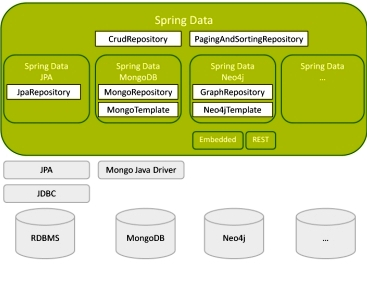
\includegraphics[width=10cm]{images/spring_data_overview}
  \caption{Architecture of Spring Data \cite{online:spring-data-overview}}
  \label{fig:spring-data-overview}
\end{figure}

\noindent JPA introduced a standard for object/relational mapping (i.e. mapping object graphs to relational database tables), with Spring Data, this support is extended to NoSQL datastores with object-like data structures.
Each type of datastore comes with its own set of annotations to provide the needed meta information for the mapping. An example of such diversity in handling different datastore mapping is reported in the code \ref{code:spring-object-mapping}.

\begin{lstlisting}[language=Java, caption=Spring Data object mapping, label=code:spring-object-mapping]
// MongoDB mapping
@Document(collection="usr")
public class User {
    @Id private String id;
    @Field("fn") private String name;
    private Date lastLogin;
    ...
}

// Neo4j mapping
@NodeEntity
public class User {
    @GraphId Long id;
    private String name;
    private Date lastLogin;
    ...
}
\end{lstlisting}

\noindent When working with data, developers generally write some DAO (Data Access Object) classes that enclose the boiler plate code for CRUD and query operations.
With JPA, CRUD operations are available through the \texttt{EntityManager} interface, queries instead needs various operations: creation, parameter set and execution.
With Spring Data, DAO classes are completely handled by the framework, requiring the user only to provide an interface of the DAO that extends a specific Spring Data repository which will map the operation to the underlying database specific implementation.
An example of this is reported in the code \ref{code:spring-dao}.

\begin{lstlisting}[language=Java, caption=Spring Data repositories, label=code:spring-dao]
public interface UserRepository extends MongoRepository<User, String> {
    List<User> findByName(String name);
    List<User> findByEmail(String email);
}
\end{lstlisting}

\subsubsection{PlayORM}
PlayORM \cite{online:playorm} is an open-source library developed by \textbf{Buffalo Software} with the aim of speeding up developer productivity of developing a NoSQL scalable solution. Currently supports Cassandra, MongoDB and HBase. 

\newparagraph PlayORM takes great inspiration from JPA interface but recognizes that JPA was designed fro DBMS and thus they have re-defined the JPA interface  for NoSQL purposes.
The framework thus make use of the JPA interfaces such as \texttt{EntityManager} for CRUD operations and the \texttt{Query} interface for queries but it re-define all the annotations.
Furthermore it defines an extensions of JPQL called S-JQL which stands for Scalable JQL that adds to JPQL the keyword \texttt{PARTITIONS} that allows the user to specify the specific data partition on which execute the query.

\noindent An example of entity defined with PlayORM is shown in the code snippet \ref{code:playorm-entity} and shows the similarities with the JPA approach.

\begin{lstlisting}[language=Java, caption=PlayORM object mapping, label=code:playorm-entity]
@NoSqlEntity
public class Employee {
    @NoSqlId
    private String id;
    private String lastName;
    @OneToOne
    private Phone phone;
    ...
}
\end{lstlisting}

\subsubsection{Apache Gora}
Apache Gora \cite{online:apache-gora} born by notice that while excellent ORM frameworks (such as JPA, Apache OpenJPA or Hibernate) exists for relational databases, data modeling in NoSQL data stores, which differ profoundly from their relational cousins, lacks of a similar tool. The aim of the project is to extend the concept of Object Relational Mapping tools (ORM), to introduce Object-to-Datastore Mapping where the underlying technological implementations rely mostly on non-relational data modeling. In essence Gora provides storage abstraction for NoSQL technologies. 
Gora thus gives the user an easy-to-use in-memory data model and persistence for big data framework with data store specific mappings and built in Apache Hadoop support.

\newparagraph The objectives of Gora can be grouped as follows:
\begin{itemize}
\item \textbf{Data Persistence}: persisting objects to Column stores such as Apache HBase, Apache Cassandra, Hypertable; key-value stores such as Voldermort, Redis, etc; SQL databases, such as MySQL, HSQLDB, flat files in local file system of Hadoop HDFS; 
\item \textbf{Data Access}: an easy to use Java-friendly common API for accessing the data regardless of its location; 
\item \textbf{Analysis}: accessing the data and making analysis through adapters for Apache Pig, Apache Hive and Cascading;
\item \textbf{MapReduce support}: out-of-the-box and extensive MapReduce (Apache Hadoop) support for data in the data store.
\end{itemize}

\subsubsection{SOS Platform}
The SOS (Save Our Systems) Platform \cite{paper:sos-platform} is a academic project developed by Unversita' Roma Tre.

\noindent The platform achieve interoperability among NoSQL databases by defining a common interface  and a meta-layer of abstraction used to maintains entities information. Database specific handlers, read the meta-layer and translate the meta-operations to database-specific operations that are finally performed over the database instance.
The architecture is shown in figure \ref{fig:sos-architecture}.

\begin{figure}[tbh]
  \centering
  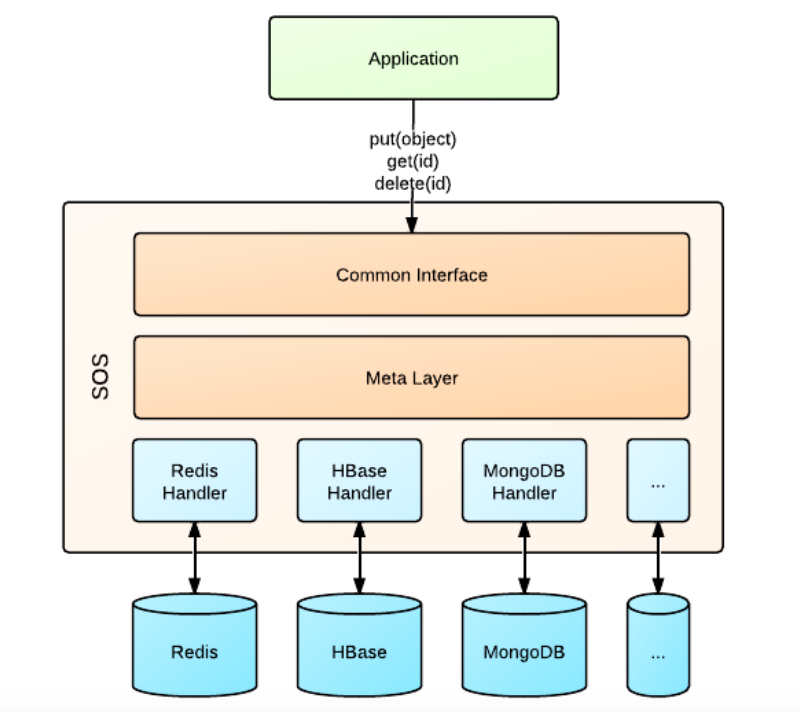
\includegraphics[width=9cm]{images/sos_architecture}
  \caption{SOS architecture \cite{paper:sos-platform}}
  \label{fig:sos-architecture}
\end{figure}

\noindent The particularity of this approach is that meta-model has been defined spotting common concepts in the model of the supported database. The meta-layer thus span among different types of NoSQL databases, in fact, three database has been chosen by the authors: Hbase to represent Column-based databases, MongoDB to represent Document-oriented databases and Redis for Key/Value stores. 

\noindent The resulting meta-layer, exploiting the models similarities, is actually very simple. It is composed by three main constructs: Struct, Set and Attribute.
Attributes contains simple values, such as Strings or Integers; Structs and Sets are instead complex elements whose values may contains both Attributes and Sets or Structs as well.
Each database is represented as a Set of collections whose is a Set itself, containing an arbitrary number of objects. Each object is identified by a key that is unique in the collections it belongs to.

\section{The JPA interface}
\label{sec:jpa}
The Java Persistence API \cite{book:projpa2} was first released as part of Enterprise JavaBeans 3.0 in 2006. As a more general-purpose object-relational mapping facility, it was quickly recognized as such, and was expanded at the request of the community to support use in Java SE environments as well as in the other Java EE container types.

\newparagraph The Java Persistence API provides an object/relational mapping facility to Java developers for managing relational data in Java applications. Java Persistence consists of three areas:
\begin{itemize}
\item the Java Persistence API;
\item object/relational mapping meta-data;
\item the query language.
\end{itemize}

\noindent Mapping meta-data are defined by the user as Java annotations upon the classes that he wants to be mapped to the underlying database.
The user annotated classes represents entities; typically an entity represents a table in a relational database, and each entity instance corresponds to a row in that table. Entities are managed by the entity manager, the EntityManager API creates and removes persistent entity instances, finds entities by the entity’s primary key, and allows queries to be run on entities. 
The \texttt{EntityManager.createQuery} and \texttt{EntityManager.createNamedQuery} methods are used to query the datastore using Java Persistence query language queries. 

\noindent The set of all entity classes managed by the \texttt{EntityManager} instance, is defined by a \textit{peristence unit}.
Persistence units are defined in the \textit{persistence.xml} configuration file, each persistence unit is identified with a name that is unique to the persistence units scope. 

\newparagraph JPA supports two methods for expressing queries to retrieve entities and other persistent data from the database: query languages and the criteria API. The primary query language is Java Persistence Query Language (JPQL), a database-independent query language that operates on the logical entity model as opposed to the physical data model. Queries may also be expressed in SQL to take advantage of the underlying database. The criteria API provides an alternative method for constructing queries based on Java objects instead of query strings.

\noindent JPQL have its roots in the Enterprise JavaBeans Query Language (EJB QL) that was first introduced in the EJB 2.0 specification to allow developers to write portable find and select methods for container-managed entity beans. It was based on a small subset of SQL and it introduced a way to navigate across entity relationships both to select data and to filter the results.
As part of JPA was then introduced JPQL that significantly extends EJB QL, eliminating many weaknesses of its father while preserving backward compatibility.

\section{Cloud Platform Independent Model}
\label{sec:cpim}
Cloud Platform Independent Model \cite{thesis:cpim} is a Java library build in order to make Java developers able to abstract their application logic from the specific Cloud Provider on which the application will actually be deployed.

\newparagraph The aim of CPIM is to overtake the vendor lock-in that affect the current PaaS industry. Each cloud provider define its own API for the services available in the PaaS environment it expose and, even if services are the same among various providers, they expose different API. This locks an application to the PaaS environment it was developed for.

\noindent Since there is no a common interface for such services, if the need of change Cloud Provider arises, maybe due to an increased cost of maintenance, the costs of re-engineer the applciation for the new Cloud provider environment dissolves the benefit of a provider migration.

\section{Summary}
In this chapter has been introduced some of the main reasons that leads to the NoSQL database definition and why industry is so interested in those kind of technology. 
\noindent Has been presented the main projects that have born trying to define a standard NoSQL language or a standard way to communicate with different NoSQL databases, giving a quick overview of the choices made by each one. 
\noindent Finally has been presented an overview of the JPA interface specification and the CPIM library, a more general approach for a common language definition in PaaS environment.
